% Copyright 2004 by Till Tantau <tantau@users.sourceforge.net>.
%
% In principle, this file can be redistributed and/or modified under
% the terms of the GNU Public License, version 2.
%
% However, this file is supposed to be a template to be modified
% for your own needs. For this reason, if you use this file as a
% template and not specifically distribute it as part of a another
% package/program, I grant the extra permission to freely copy and
% modify this file as you see fit and even to delete this copyright
% notice. 

\documentclass{beamer}
% Replace the \documentclass declaration above
% with the following two lines to typeset your 
% lecture notes as a handout:
%\documentclass{article}
%\usepackage{beamerarticle}

\usepackage{graphicx}
\usepackage{hyperref}
\usepackage[utf8]{inputenc}
\usepackage{tabto}
 
\graphicspath{ {img/} }


% There are many different themes available for Beamer. A comprehensive
% list with examples is given here:
% http://deic.uab.es/~iblanes/beamer_gallery/index_by_theme.html
% You can uncomment the themes below if you would like to use a different
% one:
%\usetheme{AnnArbor}
%\usetheme{Antibes}
%\usetheme{Bergen}
%\usetheme{Berkeley}
%\usetheme{Berlin}
%\usetheme{Boadilla}
%\usetheme{boxes}
%\usetheme{CambridgeUS}
%\usetheme{Copenhagen}
%\usetheme{Darmstadt}
%\usetheme{default}
%\usetheme{Frankfurt}
%\usetheme{Goettingen}
%\usetheme{Hannover}
%\usetheme{Ilmenau}
%\usetheme{JuanLesPins}
%\usetheme{Luebeck}
%\usetheme{Madrid}
%\usetheme{Malmoe}
%\usetheme{Marburg}
%\usetheme{Montpellier}
%\usetheme{PaloAlto}
%\usetheme{Pittsburgh}
%\usetheme{Rochester}
%\usetheme{Singapore}
%\usetheme{Szeged}
\usetheme{Warsaw}

\title{Programming with Python}

% A subtitle is optional and this may be deleted
\subtitle{Lesson 6: Flask}

%\author{F.~Author\inst{1} \and S.~Another\inst{2}}
% - Give the names in the same order as the appear in the paper.
% - Use the \inst{?} command only if the authors have different
%   affiliation.

%\institute[Universities of Somewhere and Elsewhere] % (optional, but mostly needed)
%{
%  \inst{1}%
%  Department of Computer Science\\
%  University of Somewhere
%  \and
%  \inst{2}%
%  Department of Theoretical Philosophy\\
%  University of Elsewhere}
% - Use the \inst command only if there are several affiliations.
% - Keep it simple, no one is interested in your street address.

\date{December 6th, 2016}
% - Either use conference name or its abbreviation.
% - Not really informative to the audience, more for people (including
%   yourself) who are reading the slides online

\subject{Python Lessons}
% This is only inserted into the PDF information catalog. Can be left
% out. 

% If you have a file called "university-logo-filename.xxx", where xxx
% is a graphic format that can be processed by latex or pdflatex,
% resp., then you can add a logo as follows:

% \pgfdeclareimage[height=0.5cm]{university-logo}{university-logo-filename}
% \logo{\pgfuseimage{university-logo}}

% Delete this, if you do not want the table of contents to pop up at
% the beginning of each subsection:
%\AtBeginSubsection[]
%{
%  \begin{frame}<beamer>{Outline}
%    \tableofcontents[currentsection,currentsubsection]
%  \end{frame}
%}

% Let's get started
\begin{document}

\begin{frame}
  \titlepage
\end{frame}

%\begin{frame}{Outline}
%  \tableofcontents
%  % You might wish to add the option [pausesections]
%\end{frame}

% Section and subsections will appear in the presentation overview
% and table of contents.
\section{Introduction \& Recap}

\begin{frame}{Last week's goals}
\pause
  \begin{itemize}
  \item We learnt about tuples and their uses in returning multiple values\pause
  \item We learnt about dictionaries\pause
  \item We discussed objects\pause
  \item We finished writing our own text based game!
  \end{itemize}  
\end{frame}

\section{Web Servers}

\begin{frame}{What is a web server?}

\pause
A web server is \pause something which \textbf{serves} you things. \pause \\

When you go on a website, you, the client, ask a server for something.\pause
This file could be an html document, an image or something completely different.

\end{frame}

\begin{frame}{HTTP requests}

\pause Specifically, you send the server an HTTP request. What is HTTP? \pause \\
HTTP - HyperTextTransferProtocol \pause - The protocol which the world wide web relies on \\

\pause There are many types of HTTP request. The most common two used are:
\begin{itemize}
  \item[] GET\pause \qquad gets you data from a location/service\pause
   \item[] POST\pause \qquad sends your data to a location/service
\end{itemize}

\end{frame}

\begin{frame}{A little more on HTTP}

\pause
Status code responses\pause
\begin{itemize}
  \item 200\pause
  \item 304\pause
  \item 400\pause
  \item 401\pause
  \item 403\pause
  \item 404\pause
  \item 500
  \end{itemize}

\end{frame}


\begin{frame}{APIs}

Any website you go on, you will have requested, using GET, the web page from a server somewhere. Any website is an example of a web server.\\ \pause
APIs are also examples of web servers.\\ \pause
They serve over the HTTP protocol, but instead of serving you a website, they serve information (or take in information and do something neat with it).

\end{frame}

\begin{frame}{An example}

\url{https://pokeapi.co/}

\end{frame}



\section{Flask}

\begin{frame}{Python in action: Flask}
Flask is a web framework, written in python allowing us to write web apps in python.\\ \pause

We can use it to write interactive websites or neat web services.
\end{frame}


\begin{frame}{Getting started with flask - Setting up our environment}
We first need pip. To install pip, i'd suggest googling it. It can be tricky to install (though if you're ubuntu based, apt-get install python3-pip is all you need to do ;)\\ \pause
To install flask - \textit{pip install flask}

\end{frame}

\begin{frame}{Getting started with flask - Setting up our environment}

\pause
Folder structure:
\begin{itemize}
  \item[] my-awesome-flask-app/\pause \qquad root directory of code\pause
  \item[] my-awesome-flask-app/templates/\pause \qquad directory of html to be rendered\pause
  \item[] my-awesome-flask-app/public/\pause \qquad directory of static files e.g. css \& js\pause
  \item[] my-awesome-flask-app/app.py\pause \qquad where our code will start
\end{itemize}

\end{frame}


\begin{frame}{Hello World!}

\begin{figure}[h]
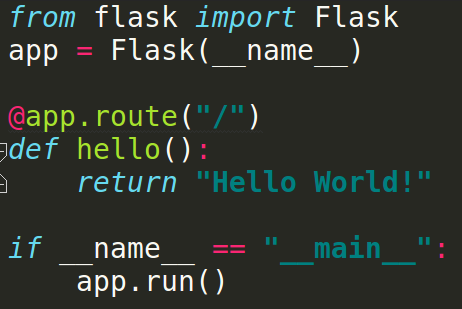
\includegraphics[width=0.9\textwidth]{flask}
\end{figure}

\end{frame}
\begin{frame}{Hello World!}

\begin{figure}[h]
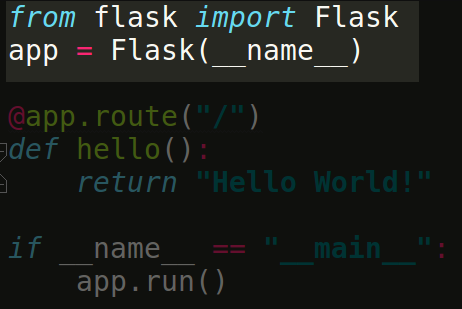
\includegraphics[width=0.9\textwidth]{flask1}
\end{figure}

\end{frame}
\begin{frame}{Hello World!}

\begin{figure}[h]
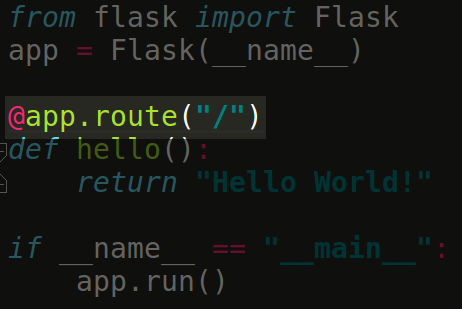
\includegraphics[width=0.9\textwidth]{flask2}
\end{figure}

\end{frame}
\begin{frame}{Hello World!}

\begin{figure}[h]
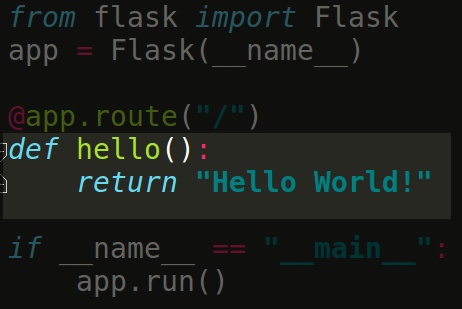
\includegraphics[width=0.9\textwidth]{flask3}
\end{figure}

\end{frame}
\begin{frame}{Hello World!}

\begin{figure}[h]
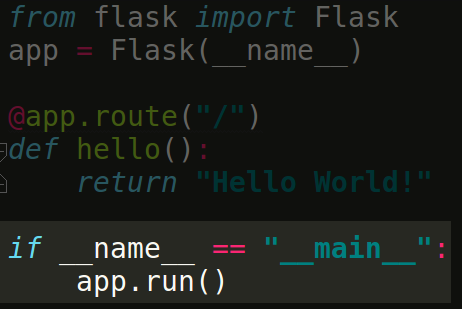
\includegraphics[width=0.9\textwidth]{flask4}
\end{figure}

\end{frame}

\begin{frame}{Endpoints}

An endpoint is a \textit{destination}. When you go to 127.0.0.1:5000 you are going to the root endpoint \textit{/}.\pause \\
If instead you go to 127.0.0.1:5000/hello/world, you are going to the endpoint \textit{/hello/world}.

\end{frame}

\begin{frame}{Templates}

Templates are pretty much HTML++.\\ \pause
They are pre-rendered on the server side and can be passed in values.

\end{frame}

\begin{frame}{Jinja2}

Flask, by default, uses the Jinja2 templating engine. It's really powerful and has some neat features.

\end{frame}

\begin{frame}{Putting everything together}

\end{frame}

\section{Summary}

\begin{frame}{That's all for tonight}
  To summarise:
  \pause
  \begin{itemize}
  \item We learnt about flask and it's ability to serve us\pause
  \item We learnt about pip and how it can help us manage packages\pause
  \item We learnt about templates and how they can render stuff for us\pause
  \item We made a neat album search tool!
  \end{itemize}
\end{frame}

\begin{frame}{THAT IS ALL}
I hope you all enjoyed our experience going through python.\\
Next semester, Amy is going to be teaching much, much more on web apps through a powerful web language, ruby on rails.\\
\end{frame}

\begin{frame}{Hope you all have a good holiday!}

\end{frame}

\end{document}


